\imagefigure{%
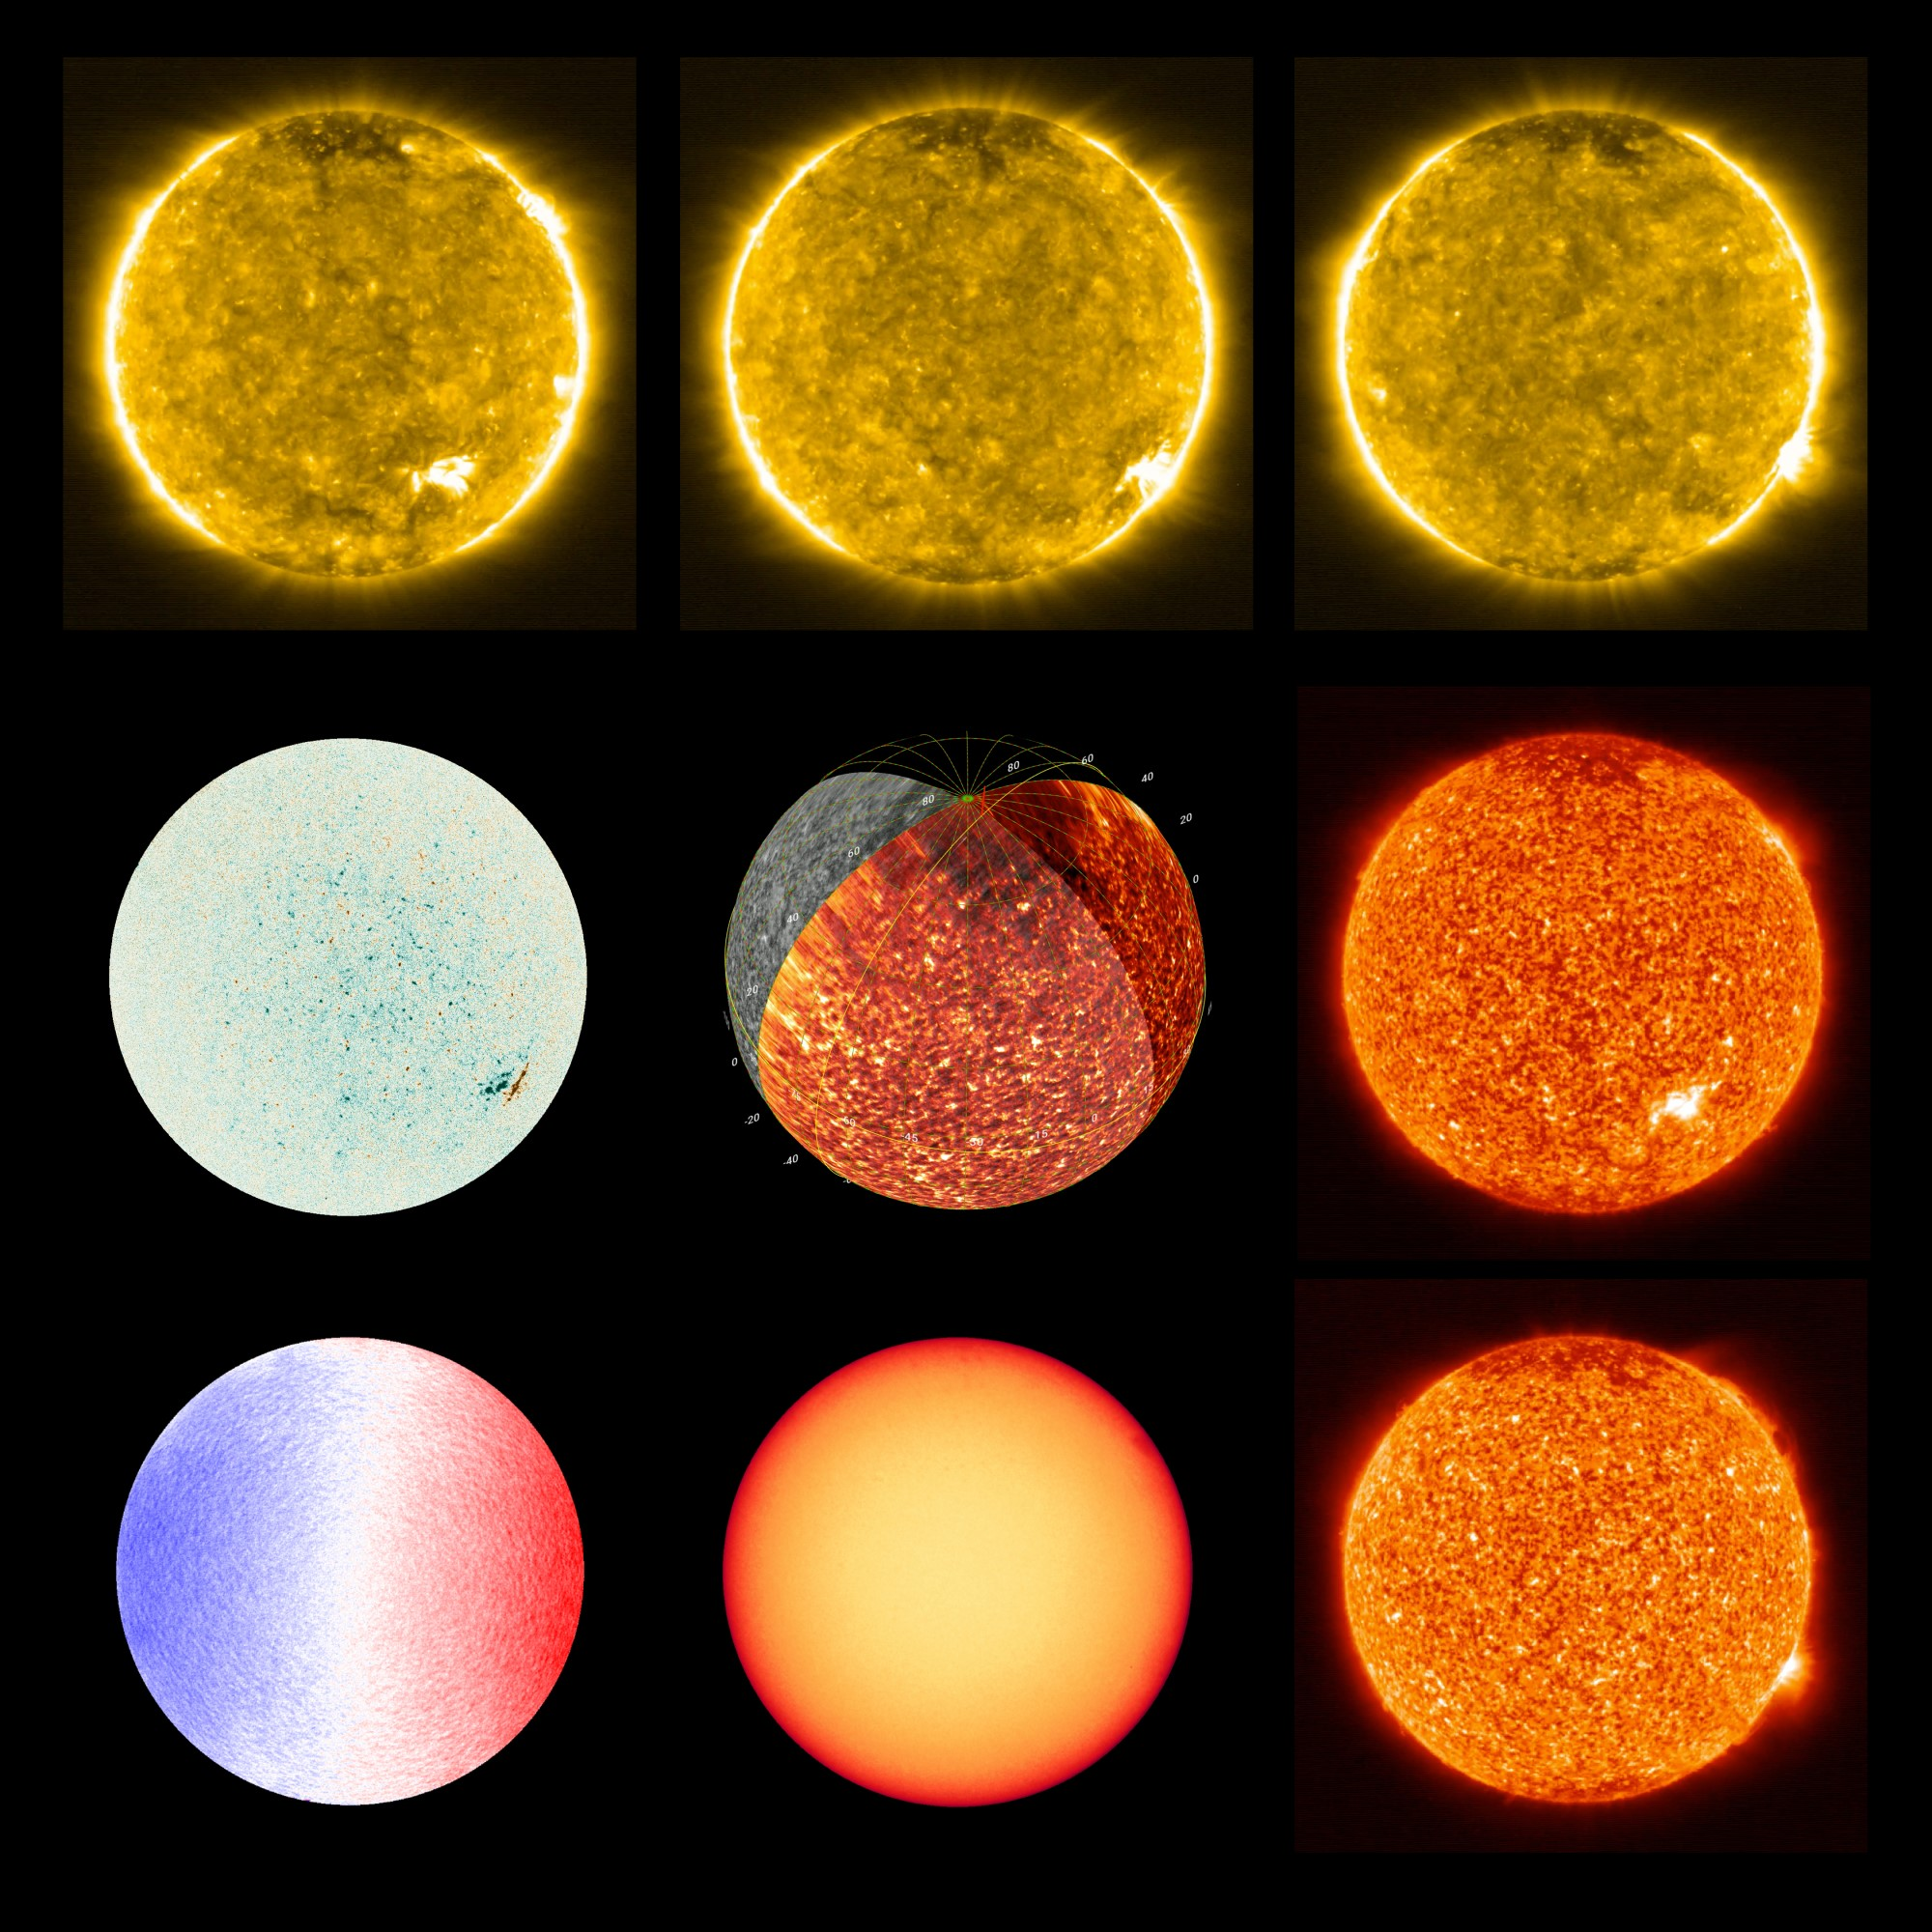
\includegraphics[width=0.85\textwidth]{10_SolarFusionQuantumTunneling/Solar_Orbiter_EUI_PHI_mosaic_FullSun_2k.jpg}
}{%
\small
\textbf{ESA's Solar Orbiter reveals multiple layers of solar activity.} This 3×3 mosaic combines images from the Extreme Ultraviolet Imager (EUI) and the Polarimetric and Helioseismic Imager (PHI) on Solar Orbiter, alongside a view from NASA's Solar Dynamics Observatory. The yellow and red panels (top row and right column) show million-degree corona and transition regions at different ultraviolet wavelengths. The center composite merges EUI and SDO views during Solar Orbiter’s first perihelion. Additional images include a PHI magnetogram of surface magnetic fields, a tachogram of solar velocities, and a visible-light image capturing a magnetically quiet Sun.
\vspace{0.5em}

\footnotesize\textit{Copyright: Solar Orbiter/EUI Team; PHI Team/ESA \& NASA}
}
